\chapter{保护生物学}\label{ch:b3:conservation-biology}

1813 年，奥杜邦曾看着一群旅鸽
连续三天飞过肯塔基上空，遮暗了天空；或许共有
五十亿只，占北美全部鸟类的四分之一。
1914 年 9 月 1 日，最后一只，一只名叫玛莎的雌鸟，死于
辛辛那提动物园。该物种在衰退开始时并不稀少；它
被成车地捕猎，其森林遭砍伐，一种
只在庞大群体中繁殖的鸟，群体一旦
稀疏到某个无人测量过的规模以下，便无法繁殖。1995 年，卡卡坡鹦鹉，
新西兰一种不会飞的夜行性鹦鹉，当时只剩五十一只；
此后每只都被命名、称重，并装上
发射器，并在恰当时机提供补充食物，
如今已有两百五十只。同年，三十一只灰
狼被放归黄石国家公园，距最后一群本地狼
被射杀已过七十年。二十年内，麋鹿迁徙，
沿河柳树重又生长，海狸也随之回归。
保护生物学是将本书所讲的种群遗传学、生态学和行为学
应用于一个实际问题——如何
防止物种消失——其算术就是
小数目的算术。

\section{小种群为何走向灭绝}

\begin{definition}[小种群的风险]\label{def:b3:conservation-biology:small}
\index{种群统计随机性}\index{环境随机性}\index{阿利效应}\index{灭绝旋涡}\index{最小可存活种群}
大种群在\omterm{prop:b3:stem-cells:gompertz}{死亡率}超过出生率时衰退；
小种群则可在两率均无变化时消失。
\emph{种群统计随机性}是指：在少数个体中，
死亡数多于出生数，或全部存活者为雄性的
机会；数十个以下时才显著。\emph{环境随机性}
——一个恶劣的冬季、一场干旱、一种疾病——同时打击每个个体，
数百个体的种群，大种群本能扛住的冲击，
可能被一扫而空；\emph{灾难}即其尾部。\emph{阿利
效应}使人均增长率在低密度时下降——配偶难寻，
群居繁殖者无处筑巢，群体难以保护
幼体，旅鸽的鸽群也无法让
捕食雏鸽的天敌饱足——因此低于阈值密度时，
种群会自行向零下降。数百个体以下时，
下一节所述的遗传过程会使适合度逐代下降；
这些因素相互促进：种群变小后，
变异减少、繁殖力下降、规模继续缩小、更易受
偶然因素冲击，并损失更多——即\emph{灭绝旋涡}
（吉尔平和苏莱，1986）。\emph{最小可存活种群}是
的规模，超过它时，给定时间跨度内灭绝的概率
（如一个世纪内 \qty{5}{\%}）可接受；
它取决于物种的生物学特性与环境的变异程度，
通常为数千个体。
\end{definition}

\begin{omfigure}
\begin{tikzpicture}[every node/.style={font=\scriptsize}, >=stealth]
  \node[draw, thick, rounded corners, fill=omThm!20, align=center] (small) at (0,0) {种群 \\变小};
  \node[draw, thick, rounded corners, fill=omDef!20, align=center] (drift) at (3.4,1.6) {遗传漂变与近交：\\变异丢失，$F$ 上升};
  \node[draw, thick, rounded corners, fill=omDef!20, align=center] (fit) at (6.8,0) {适合度下降：\\幼体减少，疾病增多};
  \node[draw, thick, rounded corners, fill=omDef!20, align=center] (chance) at (3.4,-1.6) {种群统计与环境 \\随机冲击加剧};
  \node[draw, thick, rounded corners, fill=omProp!25, align=center] (allee) at (9.9,0) {阿利效应：\\增长率为负};
  \draw[->, very thick] (small) -- (drift); \draw[->, very thick] (drift) -- (fit); \draw[->, very thick] (fit) -- (chance); \draw[->, very thick] (chance) -- (small);
  \draw[->, thick, omProp!80!black] (fit) -- (allee); \draw[->, thick, omProp!80!black] (allee.south) .. controls (9.9,-3) and (0,-3.4) .. (small.south);
  \node[align=center, font=\tiny] at (3.4,0) {灭绝旋涡：\\每一轮都使 \\种群缩小，并加速下一轮};
  \node[left, align=right, font=\tiny] at (-1.7,1.5) {栖息地丧失、过度捕获、\\入侵捕食者、疾病 \\推动种群陷入};
  \draw[->, thick, gray] (-1.6,1.2) -- (small.north west);
\end{tikzpicture}

{\small \omterm{def:b3:conservation-biology:small}{灭绝旋涡}。外部冲击使一个种群
变小；此后变异丢失，适合度降低，使
种群暴露于偶然因素之中，并使其进一步变小。保护的任务
是在环路闭合之前将其打破。}
\end{omfigure}

\begin{theorem}[有效种群大小]\label{thm:b3:conservation-biology:ne}
\index{有效种群大小}\index{性别比例}\index{调和平均数}\index{近交系数}\index{杂合度}
种群丢失变异并累积近交的速率，
并不取决于其普查规模 $N$，而取决于其
\emph{\omterm{thm:b3:conservation-biology:ne}{有效种群大小}} $N_{e}$：理想种群的大小——
种群规模恒定、随机交配、\omterm{thm:b3:conservation-biology:ne}{性别比例}相等、家庭规模服从泊松分布——这样的种群
将以相同速率丢失\omterm{thm:b3:conservation-biology:ne}{杂合度}。与理想情形的三种偏离都会
降低它。\omterm{thm:b3:conservation-biology:ne}{性别比例}不等时，设繁殖雄性有 $N_{m}$ 个，
雌性有 $N_{f}$ 个：
\[
N_{e} = \frac{4N_{m}N_{f}}{N_{m} + N_{f}} ;
\]
一只雄性与一百只雌性时，$N_{e} \approx 4$。种群规模波动时
经 $t$ 代：$N_{e}$ 为各代规模的\emph{\omterm{thm:b3:conservation-biology:ne}{调和平均数}}，
$1/N_{e} = (1/t)\sum 1/N_{i}$，由最小者主导
最小者——一个千体种群若曾降至十个，
则该时段内 $N_{e}$ 接近一百。家庭规模的方差
超过泊松分布时还会进一步降低它。在\omterm{thm:b3:conservation-biology:ne}{有效种群大小}为
$N_{e}$ 的种群中，\emph{\omterm{thm:b3:conservation-biology:ne}{近交系数}} $F$——即
个体某基因座上两个等位基因
同为一个祖先等位基因拷贝的概率——每代增加 $1/2N_{e}$，
\[
F_{t} = 1 - \Bigl(1 - \frac{1}{2N_{e}}\Bigr)^{t} \approx \frac{t}{2N_{e}},
\qquad H_{t} = H_{0}\Bigl(1 - \frac{1}{2N_{e}}\Bigr)^{t} ,
\]
而\emph{\omterm{thm:b3:conservation-biology:ne}{杂合度}} $H$ 以相同速率衰减。富兰克林的
经验法则“50/500”：$N_{e} \ge 50$ 时，每代近交
率低于 \qty{1}{\%}，这是动物育种者可接受的速率；$N_{e} \ge
500$ 则可让突变补偿漂变所消除的变异。由于 $N_{e}$
通常约为普查规模的十分之一，因此该法则要求
种群规模为五百至五千。
\end{theorem}
\begin{proof}
从种群中随机抽取的两个配子，是同一亲本等位基因的拷贝，
其概率在理想种群中为 $1/2N$，
即 $F$ 的增量；\omterm{thm:b3:conservation-biology:ne}{杂合度}以 $1 - F$ 为比例缩放，因此每代
乘以 $(1 - 1/2N_{e})$，得到指数
衰减；当 $t \ll N_{e}$ 时，$F$ 呈线性上升。\omterm{thm:b3:conservation-biology:ne}{性别比例}：一半
基因来自每一性别，因此两个配子共享一个
亲本等位基因的概率为 $\tfrac{1}{4}\cdot\tfrac{1}{2N_{m}} +
\tfrac{1}{4}\cdot\tfrac{1}{2N_{f}}$（四分之一的配对两者均为父源，
四分之一均为母源）；令其等于 $1/2N_{e}$
得 $1/N_{e} = 1/(4N_{m}) + 1/(4N_{f})$，即上式。规模波动：
经过 $t$ 代后\omterm{thm:b3:conservation-biology:ne}{杂合度}为 $H_{0}\prod(1 - 1/2N_{i})
\approx H_{0}\exp(-\sum 1/2N_{i})$，等于 $H_{0}\exp(-t/2N_{e})$
当 $1/N_{e}$ 为 $1/N_{i}$ 的平均值时。近交降低
适合度，因为它使隐性有害等位基因以
纯合子形式暴露——\emph{近交衰退}，即
存活或繁殖力下降数个百分点，
在多数异交物种中，$F$ 每增加 \qty{10}{\%}。
\end{proof}

\begin{omfigure}
\begin{tikzpicture}
\begin{axis}[
  width=0.46\linewidth, height=5.2cm,
  axis x line=bottom, axis y line=left,
  xmin=0, xmax=1, ymin=0, ymax=1.05,
  xlabel={繁殖个体中雄性所占比例}, ylabel={$N_{e}/N$},
  xlabel style={font=\small, at={(axis description cs:0.5,-0.12)}, anchor=north}, ylabel style={font=\small},
  tick label style={font=\small}, xtick={0,0.1,0.5,0.9,1}, ytick={0.36,1},
  clip=false,
]
\addplot[very thick, omDef, domain=0.005:0.995, samples=100] {4*x*(1-x)};
\draw[dashed, gray] (axis cs:0.1,0) -- (axis cs:0.1,0.36) -- (axis cs:0,0.36);
\node[font=\scriptsize, omDef, anchor=south] at (axis cs:0.5,1.0) {雌雄相等：$N_{e} = N$};
\node[font=\scriptsize, anchor=west, align=left] at (axis cs:0.12,0.2) {十只中仅一只雄性 \\参与繁殖：$N_{e} = 0.36N$};
\end{axis}
\begin{axis}[
  at={(0.5\linewidth,0)}, anchor=south west,
  width=0.46\linewidth, height=5.2cm,
  axis x line=bottom, axis y line=left,
  xmin=0, xmax=100, ymin=0, ymax=1.05,
  xlabel={代数}, ylabel={杂合度 $H_{t}/H_{0}$},
  xlabel style={font=\small, at={(axis description cs:0.5,-0.12)}, anchor=north}, ylabel style={font=\small},
  tick label style={font=\small}, xtick={0,25,50,75,100}, ytick={0.37,0.6,0.9,1},
  yticklabels={0.37,0.6,0.9,1},
  clip=false,
]
\addplot[very thick, omThm, domain=0:100, samples=60] {(1-1/20)^x};
\addplot[very thick, omMeth!70!black, domain=0:100, samples=60] {(1-1/100)^x};
\addplot[very thick, omDef, domain=0:100, samples=60] {(1-1/1000)^x};
\node[font=\scriptsize, omThm, anchor=north west] at (axis cs:12,0.55) {$N_{e} = 10$};
\node[font=\scriptsize, omMeth!70!black, anchor=south west] at (axis cs:50,0.62) {$N_{e} = 50$};
\node[font=\scriptsize, omDef, anchor=south west] at (axis cs:60,0.95) {$N_{e} = 500$};
\end{axis}
\end{tikzpicture}

{\small 左：偏斜的\omterm{thm:b3:conservation-biology:ne}{性别比例}如何缩小\omterm{thm:b3:conservation-biology:ne}{有效种群大小}——一个后宫制物种
仅十分之一的雄性参与繁殖，其 $N_{e}$ 为普查数的三分之一。右：\omterm{thm:b3:conservation-biology:ne}{杂合度}
每代按 $(1 - 1/2N_{e})$ 衰减——种群大小为十的种群
约一个世纪即丧失大部分变异，
大小为五百的种群几乎不损失。}
\end{omfigure}

\begin{proof}[证据]
佛罗里达豹在 20 世纪 90 年代仅余约二十五只，
表现出弯曲的尾巴、隐睾、心脏缺陷，精子中有
\qty{90}{\%} 为异常——近交衰退清晰可见；1995 年从得克萨斯
引入的八只雌性（\emph{遗传拯救}）使种群增至三倍，
缺陷随之减退。皇家岛狼由一对祖先于 1949 年建立并与外界隔绝，
到 2018 年衰退为两只严重近交的个体，
所检视的骨骼大多存在脊柱畸形。伊利诺伊州的大草原鹑
数量从数千只降至五十只，其卵的孵化率由 \qty{93}{\%} 降至
\qty{56}{\%}，在从其他州引入鸟只后得以恢复。
博物馆标本与古 DNA 使各案例中
\omterm{thm:b3:conservation-biology:ne}{杂合度}的损失能够直接与
衰退前的种群相比较。
\end{proof}

\begin{omfigure}
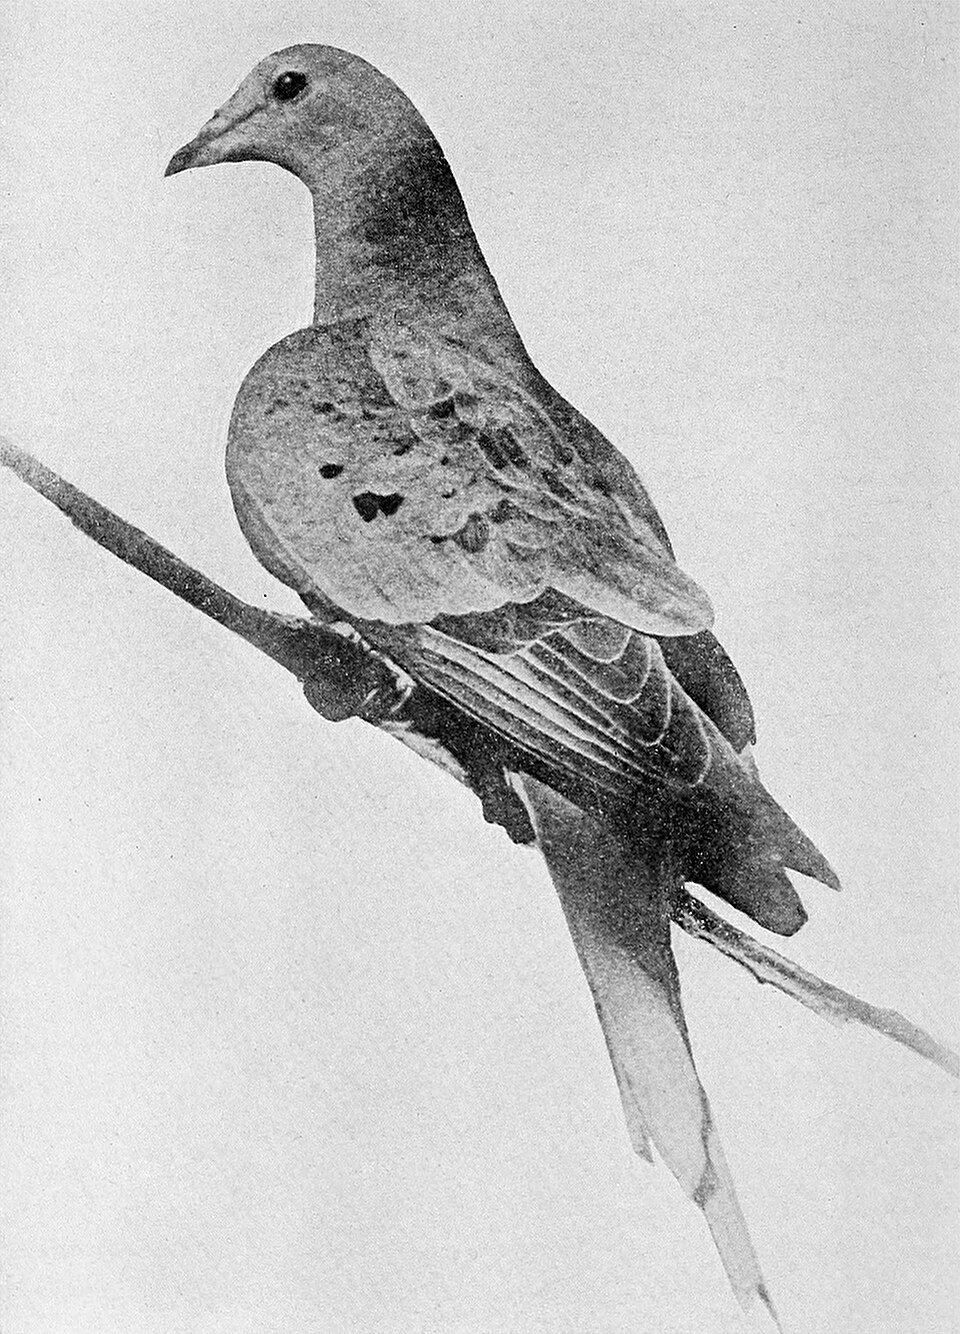
\includegraphics[width=0.4\linewidth]{images/book5/martha.jpg}\hspace{0.04\linewidth}
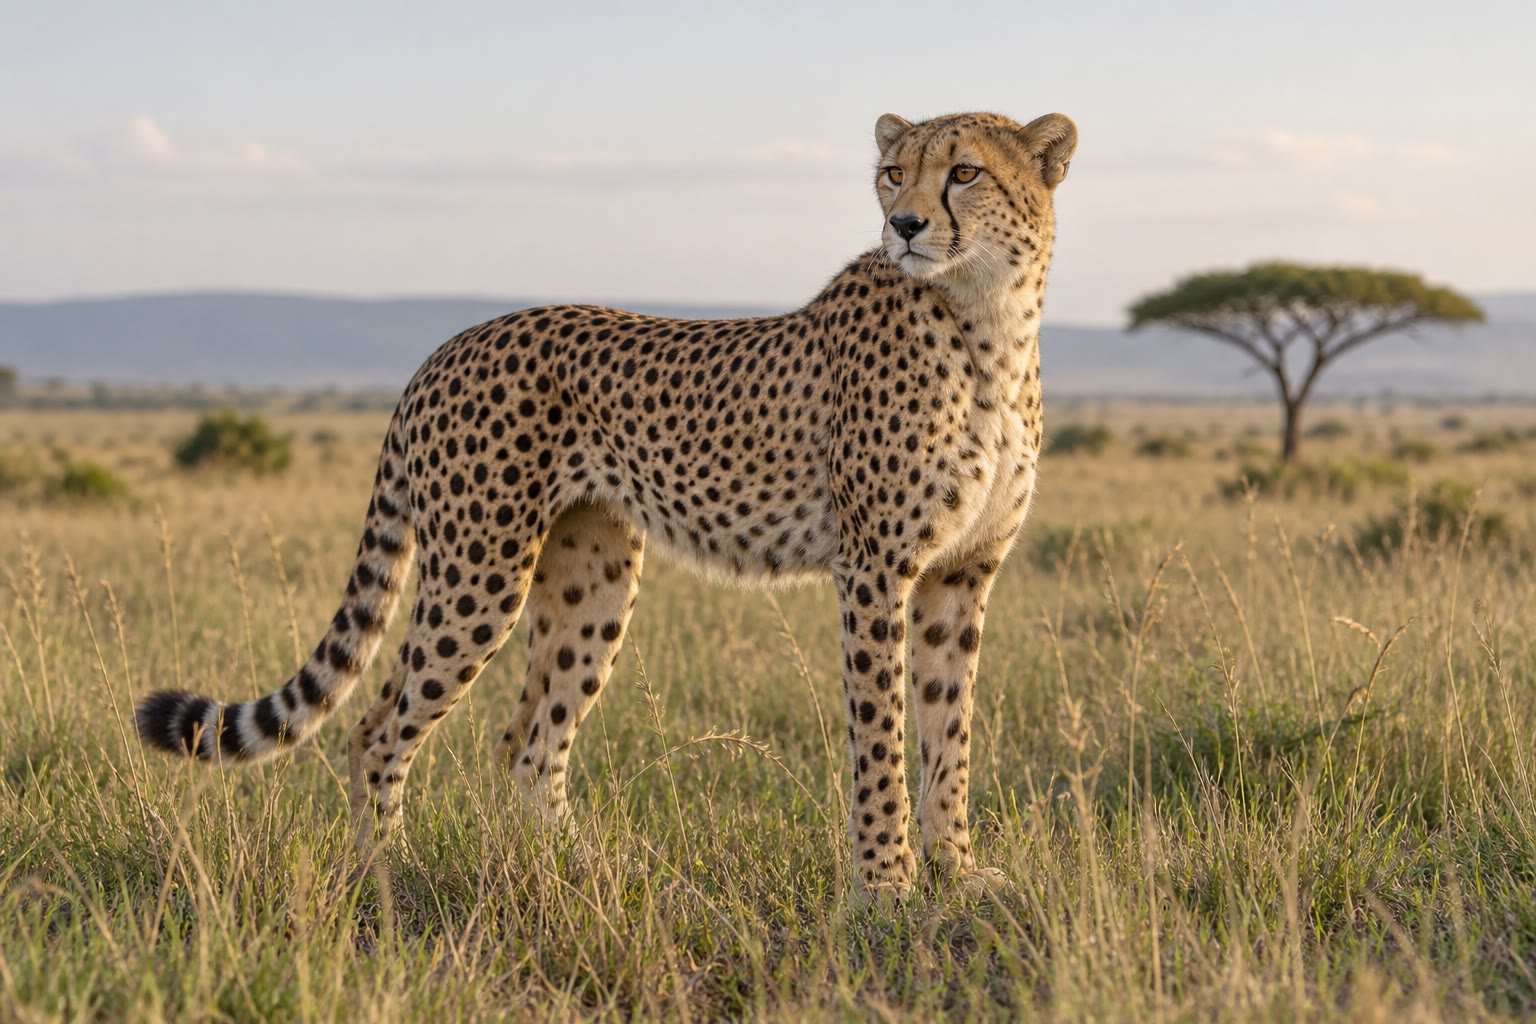
\includegraphics[width=0.52\linewidth]{images/book5/ai/b5-27-cheetah.jpg}

{\small 左：最后一只旅鸽玛莎，摄于 1912 年的
辛辛那提动物园；该物种在有记忆的年代
曾有数十亿只（照片：Enno Meyer，公有领域）。右：猎豹——
一个约一万年前经历过瓶颈的物种，
其个体之间如此相似，以至于无亲缘关系的个体之间的
皮肤移植不会被排斥。}
\end{omfigure}

\section{栖息地：多大面积，何种形状}

\begin{proposition}[物种与面积]\label{prop:b3:conservation-biology:area}
\index{物种–面积关系}\index{栖息地破碎化}\index{岛屿生物地理学}\index{廊道}\index{SLOSS 争论}\index{边缘效应}
在岛屿之间，以及在表现如同岛屿的栖息地片段之间，
物种数 $S$ 随面积 $A$ 按幂律增长，
\[
S = c\,A^{z}, \qquad z \approx 0.15\text{--}0.35,
\]
即\emph{\omterm{prop:b3:conservation-biology:area}{物种–面积关系}}（阿伦尼乌斯，1921；MacArthur 与
Wilson 的\omterm{prop:b3:conservation-biology:area}{岛屿生物地理学}，1967，将其解释为迁入与
灭绝之间的平衡，小岛上的灭绝更快）。
取 $z = 0.25$，若栖息地面积损失 \qty{90}{\%}，
最终将损失 $1 - 0.1^{0.25} = \qty{44}{\%}$ 的物种；损失一半则损失
\qty{16}{\%}。损失并非立即发生——\emph{灭绝债}
在数十年间逐步偿还，因为那些对其片段而言过小的种群逐渐萎缩——
而将固定面积\emph{破碎化}为若干片段，又会带来额外损失：
每个片段所容纳的种群更小，\emph{\omterm{prop:b3:conservation-biology:area}{边缘效应}}
（风、热、捕食者、杂草）深入森林达数百米，
而需要内部生境的物种所损失的，
超出了面积变化所能解释的部分。
对于同等总面积，是一个大保护区还是若干小保护区更能保存物种（\emph{SLOSS} 争论），
取决于物种本身：大保护区容纳更大的种群和内部生境，
小保护区则分散灾难风险，并采样到更多的生境类型。
\emph{\omterm{prop:b3:conservation-biology:area}{廊道}}使个体与基因得以在片段之间迁移，
把孤立种群转变为一个集合种群，
其各部分可在局部灭绝后重新定殖，
并能免于近交之害——这正是为何保护区之间的
土地已与保护区本身同样受到关注。
\end{proposition}
\begin{proof}
幂律是经验性的，在双对数坐标上对世界各地的群岛、湖泊、
山顶和森林片段进行拟合；对于大陆的片段，$z$ 的值较低
（迁入使物种得以留存），而对于真正的岛屿则较高。
比例损失可由此直接得出：$S'/S = (A'/A)^{z}$。\omterm{prop:b3:conservation-biology:area}{岛屿生物地理学}的机制
由 Simberloff 与 Wilson（1969）加以检验，他们对佛罗里达的
小型红树林小岛进行熏蒸，
杀灭了所有节肢动物，并观察到物种数
在一年内恢复到原先的数值——形成一种平衡，
但物种已与先前不同：数量由面积与距离决定，
而物种的身份则取决于偶然。
\end{proof}

\begin{omfigure}
\begin{tikzpicture}
\begin{loglogaxis}[
  width=0.6\linewidth, height=5.4cm,
  axis x line=bottom, axis y line=left,
  xmin=0.5, xmax=20000, ymin=5, ymax=300,
  xlabel={面积 (km$^2$)}, ylabel={物种数},
  xlabel style={font=\small, at={(axis description cs:0.5,-0.12)}, anchor=north}, ylabel style={font=\small},
  tick label style={font=\small}, xtick={1,10,100,1000,10000}, xticklabels={1,10,100,1000,10000}, ytick={10,30,100,300}, yticklabels={10,30,100,300},
  clip=false,
]
\addplot[very thick, omDef, domain=0.5:20000, samples=40] {20*x^0.25};
\addplot[only marks, mark=*, mark size=1.8pt, omDef!70!black] coordinates {(1,22) (3,24) (10,38) (30,44) (100,66) (300,80) (1000,110) (3000,150) (10000,190)};
\draw[dashed, gray] (axis cs:10000,5) -- (axis cs:10000,200) -- (axis cs:0.5,200);
\draw[dashed, gray] (axis cs:1000,5) -- (axis cs:1000,112.5) -- (axis cs:0.5,112.5);
\node[font=\scriptsize, omDef, anchor=south west] at (axis cs:1.2,215) {$S = c\,A^{0.25}$：对数坐标上的斜率 $z$};
\node[font=\scriptsize, anchor=west, align=left] at (axis cs:1200,40) {损失 \qty{90}{\%} 的面积：\\保留 $0.1^{0.25} = \qty{56}{\%}$\\的物种};
\end{loglogaxis}
\end{tikzpicture}

{\small 对数坐标上的物种–面积定律。其斜率即指数 $z$；由此可
读出栖息地缩小后物种最终的损失——森林的十分之一
约保留一半的物种，
而非线性估计给出的十分之一。}
\end{omfigure}

\begin{omfigure}
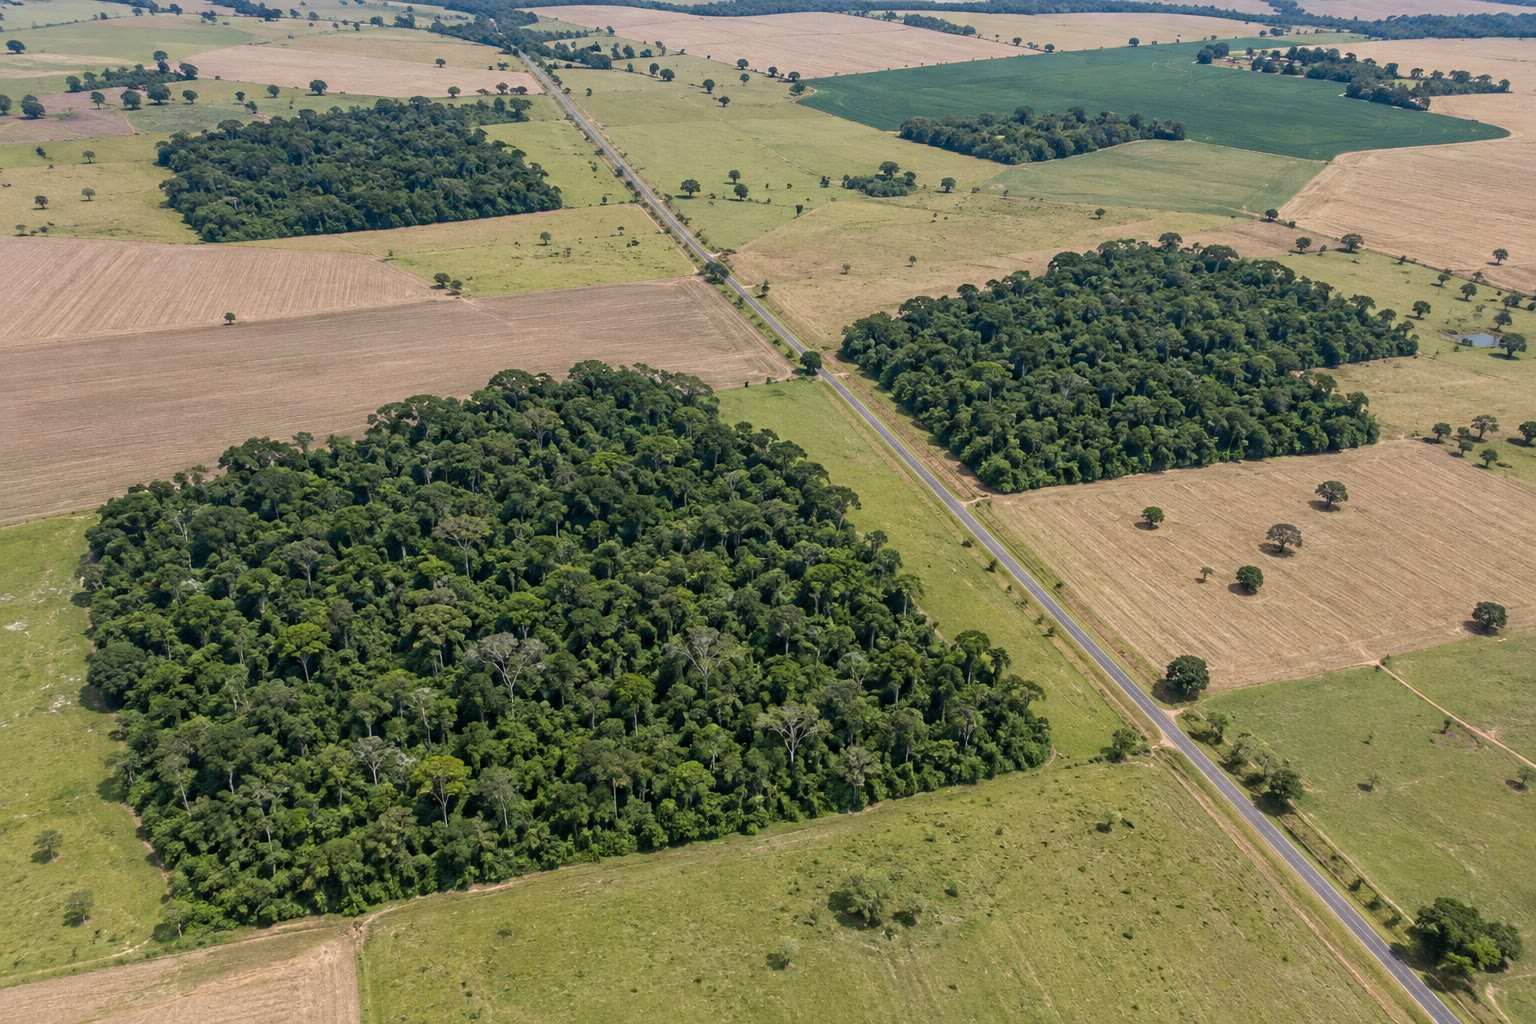
\includegraphics[width=0.6\linewidth]{images/book5/ai/b5-27-forest-fragments.jpg}

{\small 农田中的森林片段，自空中俯瞰：每个小岛所容纳的种群
都小于原先整片森林的种群，周边是内部物种无法利用的边缘带，
片段之间隔着森林物种无法穿越的
农田。}
\end{omfigure}

\section{预测与预防}

\begin{method}[种群生存力分析]\label{met:b3:conservation-biology:pva}
\index{种群生存力分析}\index{准灭绝}
用于估计种群的灭绝风险及可降低该风险的因素：
(1) 建立种群动态模型——一个由年龄或阶段特异的存活率与繁殖力构成的矩阵，
参见本科二年级分册中的种群统计学，其数据由数年间对标记个体的观测估计；
(2) 加入随机性——其一为\omterm{def:b3:conservation-biology:small}{种群统计随机性}，即逐个随机决定个体的命运，
其二为\omterm{def:b3:conservation-biology:small}{环境随机性}，即依据观测方差随机抽取每年的增长速率，
并偶发灾难；
(3) 在数据允许时加入密度依赖及近交导致的遗传衰退；
(4) 从当前大小出发，在所关心的时间范围内模拟数千条轨迹，
并记录降至
\emph{\omterm{met:b3:conservation-biology:pva}{准灭绝}}阈值（一旦低于该值即判定无法恢复）以下的比例；
(5) 改变输入参数——成体存活率、幼体存活率、栖息地面积、
迁入十只动物等——看哪一项的变化最能降低风险，
那便是应投入努力之处。输出结果是一个具有较大不确定度的概率，
而非预测；其价值在于相对比较。
分析已多次表明，在长寿物种中，决定种群命运的杠杆是成体存活率，
而非繁殖力，这也是为何延绳钓
渔业捕杀信天翁种群的速度，远快于
任何巢穴损失所能造成的影响，
尽管这些鸟每两年才产一枚卵。
\end{method}

\begin{proposition}[灭绝时间]\label{prop:b3:conservation-biology:time}
\index{灭绝时间}
对于因环境变化而波动的种群，设其平均增长速率 $\bar r$ 接近零，
年增长速率的方差为 $\sigma^{2}$，
则种群大小的对数构成一个带漂移的随机游走，
从大小为 $N$ 出发的期望\omterm{prop:b3:conservation-biology:time}{灭绝时间}，
仅随 $N$ 的\emph{对数}增长（条件为 $\bar r < 0$）——种群加倍只增加固定的若干年，
而随 $N$ 的\emph{幂}增长（条件为 $\bar r > 0$），
指数为 $2\bar r/\sigma^{2} - 1$；若仅考虑\omterm{def:b3:conservation-biology:small}{种群统计随机性}，则它随种群大小以\emph{指数}方式增长，
因此，在 $N$ 为一百时对种群统计偶然性安全的种群，
在一万个个体时仍可能因环境方差而消失。
实际的推论是：降低种群增长的方差——
通过增加栖息地、增加栖息地点位、拓宽食谱等方式，
缓冲坏年景的冲击——对其持续存在的作用，
可能比提高其平均
增长速率更大。
\end{proposition}
\admitted

\begin{omfigure}
\begin{tikzpicture}
\begin{semilogyaxis}[
  width=0.62\linewidth, height=5.4cm,
  axis x line=bottom, axis y line=left,
  xmin=0, xmax=50, ymin=1, ymax=3000,
  xlabel={年}, ylabel={种群大小},
  xlabel style={font=\small, at={(axis description cs:0.5,-0.12)}, anchor=north}, ylabel style={font=\small},
  tick label style={font=\small}, xtick={0,10,20,30,40,50}, ytick={1,10,100,1000}, yticklabels={1,10,100,1000},
  clip=false,
]
\addplot[thick, omDef] coordinates {(0,200) (2,240) (4,190) (6,260) (8,300) (10,220) (12,180) (14,250) (16,330) (18,280) (20,350) (22,300) (24,260) (26,340) (28,420) (30,380) (32,450) (34,400) (36,520) (38,480) (40,560) (42,500) (44,600) (46,650) (48,610) (50,700)};
\addplot[thick, omThm] coordinates {(0,200) (2,150) (4,180) (6,120) (8,90) (10,110) (12,70) (14,50) (16,60) (18,35) (20,40) (22,25) (24,18) (26,22) (28,12) (30,8) (32,9) (34,5) (36,3) (38,2) (40,1)};
\addplot[thick, omMeth!70!black] coordinates {(0,200) (2,210) (4,170) (6,200) (8,140) (10,160) (12,120) (14,140) (16,90) (18,110) (20,80) (22,95) (24,60) (26,75) (28,50) (30,55) (32,40) (34,45) (36,30) (38,35) (40,28) (42,30) (44,22) (46,25) (48,20) (50,22)};
\draw[dashed, gray] (axis cs:0,20) -- (axis cs:50,20); \node[font=\scriptsize, gray, anchor=north east] at (axis cs:49,18) {准灭绝阈值};
\node[font=\scriptsize, omDef, anchor=west] at (axis cs:50.5,700) {$\bar r > 0$：持续存在};
\node[font=\scriptsize, omMeth!70!black, anchor=west] at (axis cs:50.5,22) {$\bar r \approx 0$：缓慢下降};
\node[font=\scriptsize, omThm, anchor=west] at (axis cs:40.5,1.3) {$\bar r < 0$：40 年内消失};
\end{semilogyaxis}
\end{tikzpicture}

{\small 从相同的两百只动物出发模拟的三条轨迹，
仅平均增长速率不同；\omterm{met:b3:conservation-biology:pva}{种群生存力分析}会运行数千次此类模拟，
并统计其中穿越阈值的次数。
逐年变化的方差，使即便是居中的情形也成为一场
赌博。}
\end{omfigure}

\begin{definition}[工具]\label{def:b3:conservation-biology:tools}
\index{IUCN 红色名录}\index{入侵物种}\index{迁地保护}\index{圈养繁殖}\index{重引入}\index{再野化}\index{营养级联}
\emph{IUCN 红色名录}依据定量标准对物种进行分类：
在十年或三代内减少 \qty{30}{\%}、\qty{50}{\%} 或 \qty{80}{\%}，
分布范围小于 \qty{20000}{}、\qty{5000}{} 或
\qty{100}{km^2}，成熟个体数低于 \qty{10000}{}、\qty{2500}{} 或
\qty{250}{}，或模型估计的灭绝概率，满足其一即可将物种
列为易危、濒危或极危；
其中四分之一的哺乳动物与八分之一的鸟类符合条件。造成物种濒危的原因
首先是栖息地丧失，其次是过度捕获、\emph{入侵物种}
（被带到其物种从未与之相遇的岛屿上的捕食者与竞争者：
老鼠、猫和臭鼬几乎夺走了新西兰的大部分鸟类，
一种棕树蛇则使关岛的大部分鸟类消失），污染
以及气候变化。应对措施包括：保护区覆盖陆地的六分之一；
控制或根除入侵者（一百五十个
岛屿已清除老鼠）；\emph{迁地保护}——种子库
在北极永久冻土中的库房里保存一百万份种质，
冷冻胚胎，以及\emph{圈养繁殖}，依据系谱图管理，
以尽量减少亲缘关系，由此使加州神鹰在 1987 年
从二十二只个体中得以恢复，黑足雪貂则从十八只个体中恢复；
\emph{重引入}，其成功率约为三分之一，
当导致最初丧失的原因已被消除时往往更高；以及
\emph{再野化}，即大型动物及其所驱动过程的回归——
黄石公园的狼，其捕食及对捕食的恐惧，使麋鹿离开河岸，
从而让柳树、白杨、海狸和鸣禽重新出现，
这一\emph{营养级联}从食肉动物一直延伸到
河流的形态。
\end{definition}

\begin{omfigure}
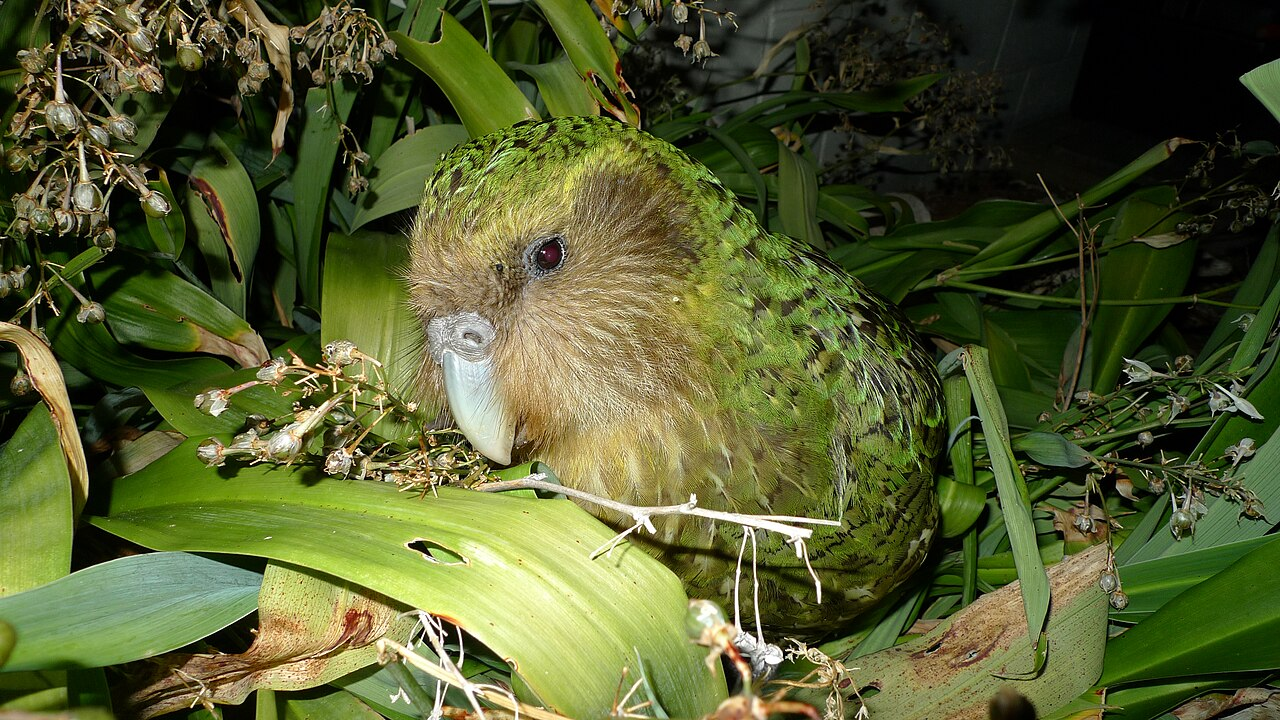
\includegraphics[width=0.46\linewidth]{images/book5/kakapo-sirocco.jpg}\hspace{0.04\linewidth}
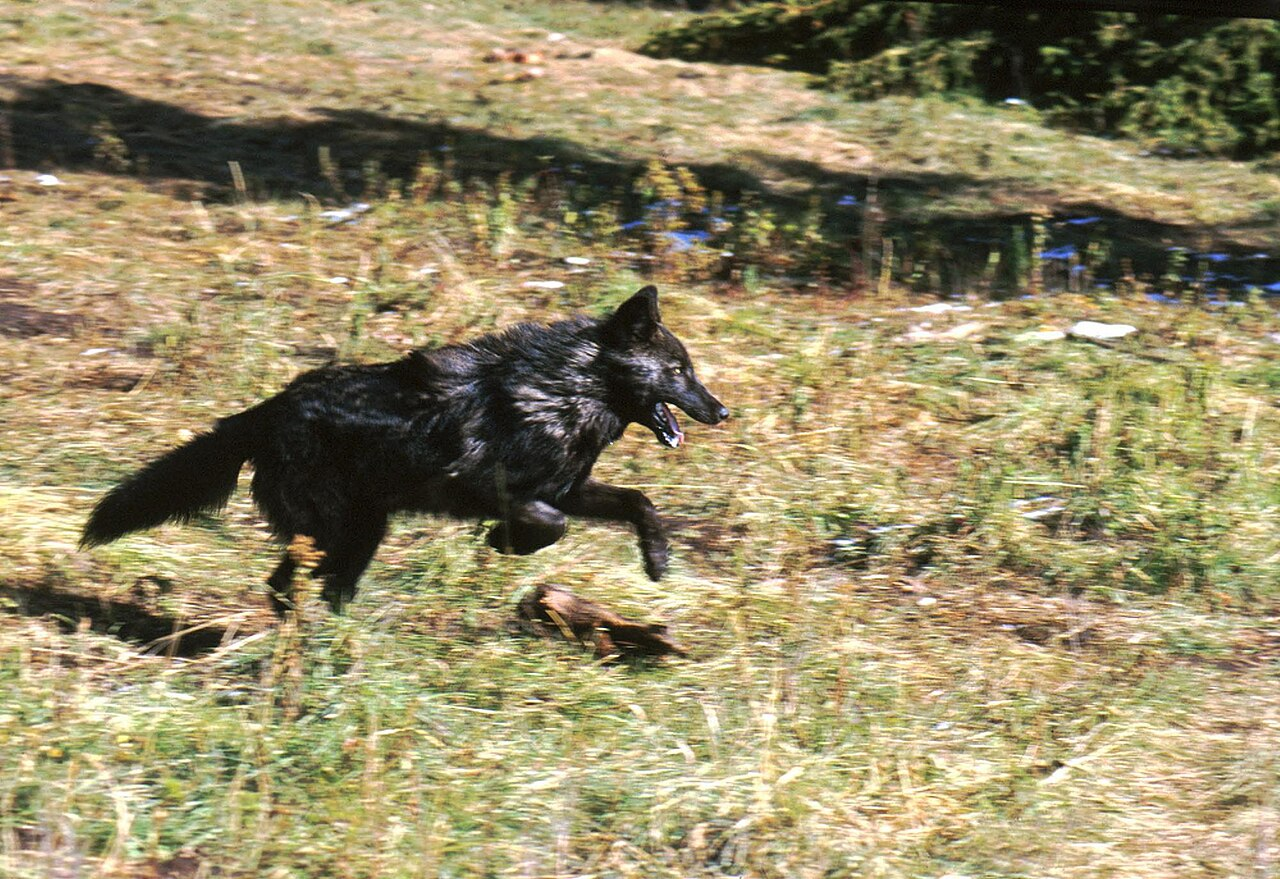
\includegraphics[width=0.46\linewidth]{images/book5/yellowstone-wolves-1996.jpg}

{\small 左：Sirocco，一只卡卡坡鹦鹉——1995 年仅存的五十一只之一，
如今约二百五十只之一，每只都有名字并受到监测，
均生活在无捕食者的岛屿上（照片：Department of Conservation, New
Zealand, CC BY 2.0）。右：1996 年黄石公园的狼，
为其\omterm{def:b3:conservation-biology:tools}{重引入}后的第一个冬天（照片：National Park Service，
公有领域）。}
\end{omfigure}

\begin{example}[三次恢复]\label{ex:b3:conservation-biology:recoveries}
卡卡坡鹦鹉：1995 年仅有五十一只，全部迁至已清除捕食者的岛屿；
每只鸟都佩戴发射器，每个巢都由照相机监视，
母鸟失职时雏鸟由人工饲养，
雄鸟在新西兰红松结果的年份被投喂，使其进入繁殖状态，
种群的系谱图得到管理，以保留最后一只菲奥尔德兰雄鸟的稀有基因；
每只卡卡坡鹦鹉的基因组都已测序。
如今有二百五十只，基因组显示其 $N_{e}$ 约为一百。
美洲鹤：1941 年仅十五只，为单一迁徙群体，
由野外鸟巢取得的卵在圈养条件下繁育，
借超轻型飞机训练其学习新的迁徙路线，如今
约八百只。座头鲸：曾被猎杀至仅剩数千只，1966 年受到保护，
如今已超过十万只，年增幅接近 \qty{8}{\%}，
这表明长寿动物在其衰退的单一原因被消除时会如何恢复。
每一次恢复耗资数千万、历时数十年；
本章的算术说明了为何须在数量降至\omterm{def:b3:conservation-biology:small}{灭绝旋涡}之前付出努力，
以及为何这比任何之后的拯救
都更为经济。
\end{example}

\begin{omfigure}
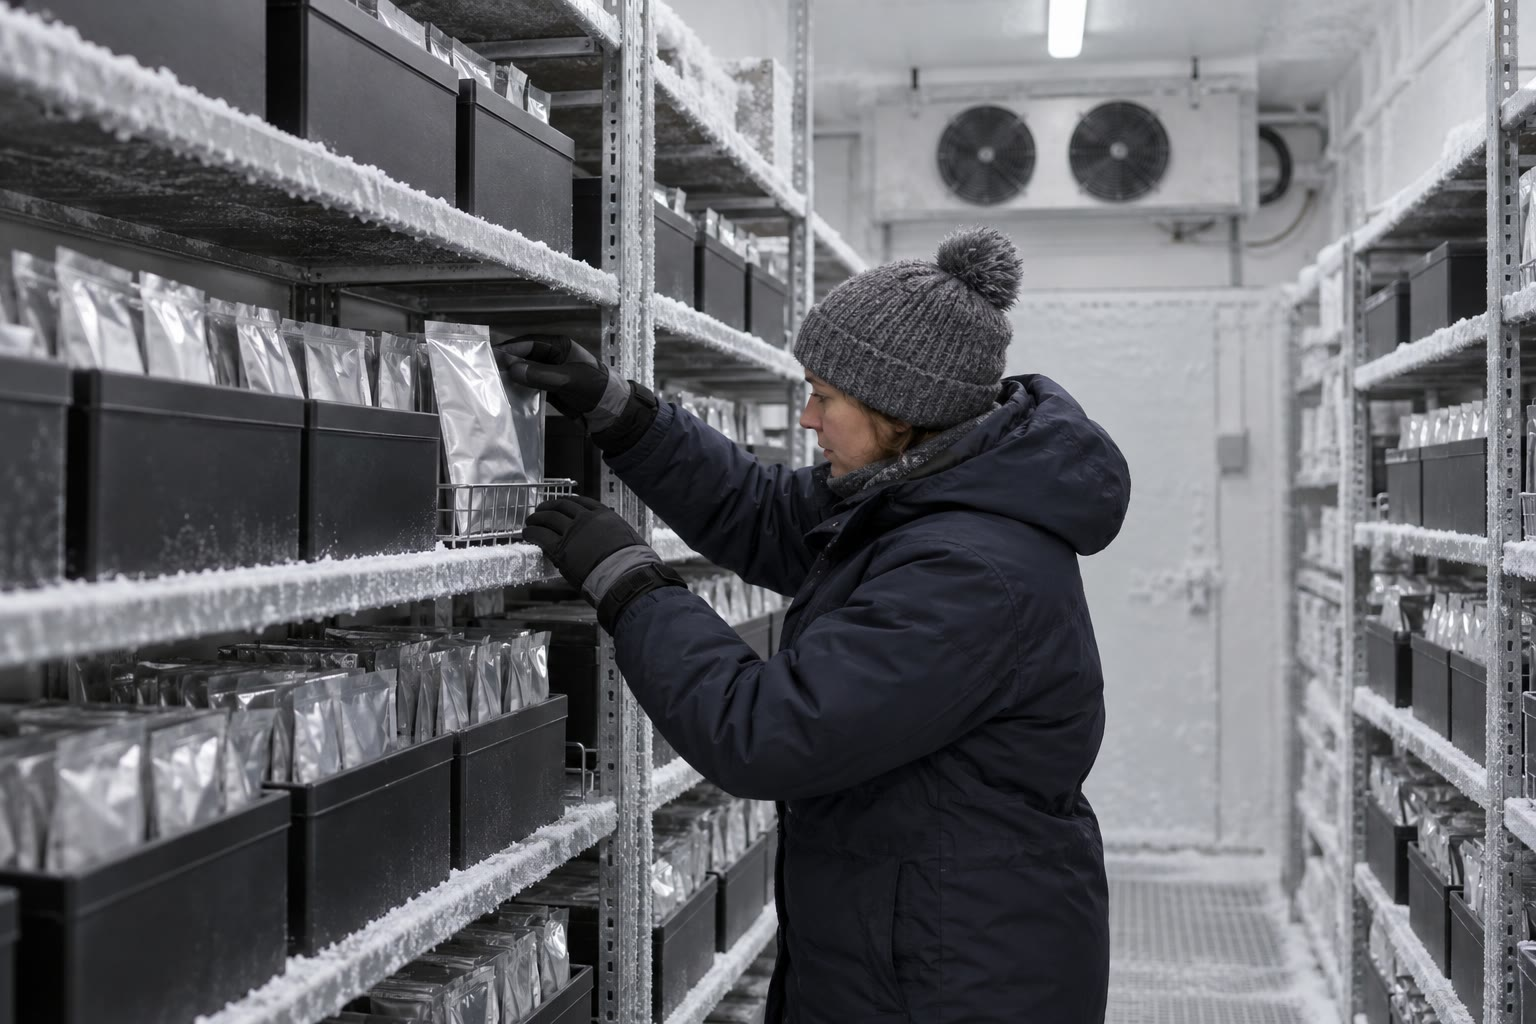
\includegraphics[width=0.56\linewidth]{images/book5/ai/b5-27-seed-vault.jpg}

{\small 位于永久冻土中的种子库：保存着百万份作物及野生植物种质材料的副本，
保存于 \qty{-18}{\celsius}，以防其所源自的收藏遭受损失——
这是一种保险式的保护，
其规模相当于一个物种的基因组。}
\end{omfigure}

\begin{remark}[保存的算术]\label{rem:b3:conservation-biology:remark}
本课程的每一章都以一个数字收尾，而本章则以若干数字收尾：
\omterm{thm:b3:conservation-biology:ne}{有效种群大小}，\omterm{thm:b3:conservation-biology:ne}{近交系数}每世代增加
$1/2N_{e}$，指数 $z$ 将损失的公顷数转化为损失的物种数，
以及一个世纪内的灭绝概率。它们都很粗略——普查并不精确，
方差多为推测，模型也是一种漫画式的简化——
但正是它们把对濒危鸟类的感慨转化为关于购买哪五十公顷土地、
迁移哪八只动物的决策。这里的生物学与本书其余部分的生物学相同：
\omterm{thm:b3:molecular-evolution:neutral}{遗传漂变}、选择、种群统计学、行为，以及种群对其栖息地、
栖息地对其种群的依赖。
唯一的新内容是紧迫性，以及这样一个事实：
这一实验只能进行一次，没有对照，
而对象正是
那些仍然存活的物种。
\end{remark}

\section{练习}

\begin{exercise}[$\star$]\label{exo:b3:conservation-biology:1}
定义\omterm{def:b3:conservation-biology:small}{种群统计随机性}、\omterm{def:b3:conservation-biology:small}{环境随机性}和\omterm{def:b3:conservation-biology:small}{阿利效应}，
并从本章中各举一例。
\end{exercise}

\begin{exercise}[$\star$]\label{exo:b3:conservation-biology:2}
什么是\omterm{thm:b3:conservation-biology:ne}{有效种群大小}？列出真实种群中使其小于普查数量的
三个特征。
\end{exercise}

\begin{exercise}[$\star$]\label{exo:b3:conservation-biology:3}
叙述物种–面积定律。若 $z = 0.25$，则栖息地在损失一半面积后，
保留的物种比例是多少？损失十分之九呢？
损失百分之九十九呢？
\end{exercise}

\begin{exercise}[$\star$]\label{exo:b3:conservation-biology:4}
解释 50/500 规则，以及每个数字各自防范的是什么。
\end{exercise}

\begin{exercise}[$\star\star$]\label{exo:b3:conservation-biology:5}
一群 200 头象海豹，其中有 8 头繁殖雄性和 120 头繁殖雌性。
计算 $N_{e}$ 以及每世代\omterm{thm:b3:conservation-biology:ne}{杂合度}的损失。
需要多少世代才会损失其四分之一？
\end{exercise}

\begin{exercise}[$\star\star$]\label{exo:b3:conservation-biology:6}
某种群在连续五个世代中的数量依次为 1000、1000、20、1000、1000。
计算该时段内的 $N_{e}$ 及保留的\omterm{thm:b3:conservation-biology:ne}{杂合度}，
并与恒定为 1000 的情形作比较。
\end{exercise}

\begin{exercise}[$\star\star$]\label{exo:b3:conservation-biology:7}
二十五只佛罗里达美洲狮，$N_{e} \approx 10$：5 个世代内积累了多少近交？若适合度下降 \qty{5}{\%}，
是每 \qty{10}{\%} 的 $F$ 所致，则适合度总计下降多少？
在下一世代中加入八只无亲缘关系的雌性，
会使 $F$ 发生什么变化？
\end{exercise}

\begin{exercise}[$\star\star$]\label{exo:b3:conservation-biology:8}
黄石公园：1995--96 年放归 31 只狼，2003 年园内约有 100 只。
估算 $r$；若增长持续，2020 年将有多少只？
为何并未如此？
\end{exercise}

\begin{exercise}[$\star\star$]\label{exo:b3:conservation-biology:9}
依据本章中的 IUCN 标准对下列情形分类：(a) 一种青蛙，其种群
十年内下降 \qty{60}{\%}；(b) 一种植物，有 180 株成熟个体；
(c) 一种鱼，其分布范围为 \qty{3000}{km^2}；(d) 一种鸟，
个体数为 \num{30000}，每十年下降 \qty{10}{\%}。
\end{exercise}

\begin{exercise}[$\star\star\star$]\label{exo:b3:conservation-biology:10}
一个由 $N$ 对组成的种群，每对以概率 $1/2$ 产生两个
存活后代，否则不产生后代（\omterm{def:b3:conservation-biology:small}{种群统计随机性}）。
计算整个种群在一代内灭绝的概率，
分别对 $N = 2$、$5$、$10$、$20$ 求出，并说明
种群统计风险如何随 $N$ 变化。
\end{exercise}

\begin{exercise}[$\star\star\star$]\label{exo:b3:conservation-biology:11}
取物种—面积律中 $z = 0.25$，将一片森林切分为 10 块面积相等、
彼此隔离的片段。比较单个片段中预期的物种数与原面积十分之一时的
物种数，并论证各片段物种数之和为何不简单等于原森林的
物种数——是什么决定了这些片段合起来
比原整体保有更多还是更少的物种？
\end{exercise}

\begin{exercise}[$\star\star\star$]\label{exo:b3:conservation-biology:12}
为何每代增加少量迁入（$m N_{e} \approx 1$）
便能在很大程度上阻止小种群中变异的丧失，
它在局部适应方面付出了什么代价？利用漂变（$1/2N_{e}$）与
迁入替换的等位基因比例（$m$）之间的平衡进行论证。
\end{exercise}

\section{问题：五十与五百}

\begin{problem}[{周末问题——一项种群挽救计划的数字：
一个被挽救的鹦鹉种群的有效大小及其近交，一次遗传挽救，
一片萎缩的森林所能保留的物种，\omterm{def:b3:conservation-biology:tools}{重引入}狼的增长，
各类别与成本，最终落在 $N_{e}$、十代之后的\omterm{thm:b3:conservation-biology:ne}{近交系数}
以及所保留物种的比例上}]
\label{pb:b3:conservation-biology:1}
数据：一个鹦鹉种群有 60 只成体，其中雄性 20 只、雌性 40 只，全部参与繁殖；
世代时间为 \qty{10}{yr}。过去五代的种群历史：
500、100、60、51、60。近交衰退：
每增加 \qty{0.1}{} 的 $F$，适合度下降 \qty{6}{\%}。挽救：10
只无亲缘关系的鸟加入 60 只。森林：面积由 \qty{2000}{km^2} 减至
\qty{300}{km^2}，$z = 0.25$；现有物种 180 种。狼：放归 31 只，
8 年后为 100 只，园内环境容纳量约 120。成本：鹦鹉每年
四百万美元。

\medskip
\noindent\textbf{第一部分——有效大小。}
\begin{enumerate}
  \item 由当前 60 只的\omterm{thm:b3:conservation-biology:ne}{性别比例}求 $N_{e}$，并与
        普查数相比较。
  \item 对过去五代取 $N_{e}$ 的调和平均；
        哪一代起主导作用？
  \item 计算这五代中积累的\omterm{thm:b3:conservation-biology:ne}{近交系数}，
        利用调和平均 $N_{e}$（给出精确公式与线性近似）。
  \item 计算由该近交造成的适合度损失。
  \item 五代之后保留的\omterm{thm:b3:conservation-biology:ne}{杂合度}，
        以原始值的比例表示。
  \item 若种群现维持在 60 只且\omterm{thm:b3:conservation-biology:ne}{性别比例}不变，
        再经十代后 $F$ 将达到多少，
        适合度损失又是多少？这需要多少年？
\end{enumerate}

\medskip
\noindent\textbf{第二部分——挽救。}
\begin{enumerate}[resume]
  \item 十只无亲缘关系的鸟加入这 60 只，下一代中来自新个体的
        等位基因比例约为 $10/70$；
        若一方亲本为本地个体、另一方为新个体，其后代的\omterm{thm:b3:conservation-biology:ne}{近交系数}
        为 $0$。若交配是随机的，估计
        下一代种群的平均 $F$。
  \item 解释为何 $F$ 会立即下降，而\omterm{thm:b3:conservation-biology:ne}{杂合度}只有在
        迁入者的等位基因扩散之后才会上升，
        并说明为何可能还需要第二次挽救。
  \item 若要以相等的\omterm{thm:b3:conservation-biology:ne}{性别比例}使 $N_{e} = 500$，
        需要多少成体？若以 $r = \qty{0.05}{yr^{-1}}$ 从 70 只鸟开始，
        需要多少年？
  \item 该计划将弱小母鸟的卵取走进行人工育雏，
        从而提高每对成功出飞雏鸟的平均数，但使家庭规模趋于一致。
        为何家庭规模趋于一致会\emph{提高}
        $N_{e}$ 使其高于普查数（趋近 $2N$）？
  \item 南方一个独特谱系中的最后一只雄性在
        野外不育。请提出两种干预措施，并说明它们对
        基因库的代价。
  \item 以每年四百万美元的成本，在 40 年内使
        $N_{e} = 500$，求总成本与每增加一只鸟的成本。这是否昂贵？
        与什么相比？
\end{enumerate}

\medskip
\noindent\textbf{第三部分——森林。}
\begin{enumerate}[resume]
  \item 求森林在 \qty{300}{km^2} 时能保留的物种比例；
        预期物种数，以及灭绝债务（即现存但将会
        丧失的物种数）。
  \item 若 \qty{300}{km^2} 改为三块彼此隔离的片段，
        每块 \qty{100}{km^2}，求每块片段的物种数；
        若各片段物种完全不同，求总数；若完全相同，求总数。
        什么决定了结果？
  \item 一条 \qty{20}{km^2} 的走廊连接这三块片段，将其
        视为一个 \qty{320}{km^2} 的区域：求预期物种数，并与
        第 14 题中物种完全相同的情形作比较。
  \item 森林中最大的捕食者每对需要 \qty{50}{km^2}，且
        需要 $N_{e}$ 为 50 才能存续。整个 \qty{300}{km^2} 能否容纳它？
        单个片段能否？这对面积与物种数作为
        标准各说明了什么？
  \item 估算灭绝债务需要多长时间才能偿还，前提是
        所损失物种的种群以每年 \qty{3}{\%} 的速率
        从 200 下降至\omterm{met:b3:conservation-biology:pva}{准灭绝}阈值 10。
  \item 为何破碎化带来\omterm{prop:b3:conservation-biology:area}{边缘效应}时，物种—面积律会低估损失，
        而当周围土地部分可利用时，
        则会高估损失？
\end{enumerate}

\medskip
\noindent\textbf{第四部分——狼与名录。}
\begin{enumerate}[resume]
  \item 狼：$r$ 由 $31 \to 100$（8 年）求出，以及倍增时间。
  \item 趋向 $K = 120$ 的逻辑斯谛增长：8 年后的种群数量
        在逻辑斯谛增长而非指数增长下，从 31 只出发，
        取第 19 题中的 $r$（用 $N(t) = K/[1 + (K/N_{0} -
        1)\mathrm{e}^{-rt}]$）。哪一种模型更符合观测到的 100 只？
        这说明早期阶段的密度制约如何？
  \item 麋鹿在 1995 年有 \num{17000} 只，2015 年有 \num{4000} 只。
        求年均下降速率。在 100 只狼的条件下，狼每年每只捕食
        \num{20} 只麋鹿，这能解释其中多少？
  \item 依据 IUCN 标准对鹦鹉（60 只成熟个体）及挽救前的
        森林捕食者进行分类。
  \item 旅鸽：1800 年约有五十亿只，1914 年灭绝。若
        自 1870 年（当时仍有数十亿只）起数量呈指数下降，
        直至 1914 年仅剩一只，则由此推出的年下降速率为多少？
        为何\omterm{def:b3:conservation-biology:small}{阿利效应}使最后几十年的下降快于
        指数速度？
  \item 用一段文字解释，为何\omterm{met:b3:conservation-biology:pva}{种群生存力分析}（PVA）在 1850 年会判断
        旅鸽是安全的，以及它会遗漏什么。
  \item 总结：当前 $N_{e}$（第 1 题），
        保持 60 只时再经十代后的 $F$（第 6 题），以及
        萎缩后的森林所保留的物种比例（第 13 题）。
\end{enumerate}
\end{problem}
